\pdfoutput=1
\RequirePackage{amsmath}
\documentclass{emulateapj}
\usepackage[varg]{newtxmath}
\usepackage{newtxtext}
\usepackage[english,spanish,es-minimal]{babel}
\usepackage[utf8]{inputenc}
\usepackage{natbib}
\usepackage{microtype}
\usepackage{hyperref}
\graphicspath{ {figs/}, {../}, {../luis-programas}}


%% Commands for the postage stamp images
\setlength{\fboxsep}{0pt}%
\newlength\figwidth
\setlength\figwidth{0.32\textwidth}
\newlength\figstampcolsep
\setlength\figstampcolsep{5pt}
\newcommand\BowshockFig[2]{
  \includegraphics[width=\figwidth, clip, trim=60 50 100 50]
  {j8oc#2010_wcs/#1-Bally_#2-images}
}
\newcommand\MissingFig[2]{%
  \framebox{\makebox[\figwidth][c]{\raisebox{0.25\figwidth}[0.48\figwidth]{%
        Not found: #1 from Field #2}}}%
}
\newcommand\raiselabel[1]{\raisebox{0.5\figwidth}[-0.5\figwidth]{#1}}


\begin{document}
\title{
  An Atlas of Stationary Bow Shock Arcs in the Orion Nebula
}
\author{
  William J. Henney, 
  Luis A. Gutiérrez-Soto,
  Jorge A. Tarango-Yong 
}

\affil{%
  \foreignlanguage{spanish}{Centro de Radioastronomía y
    Astrofísica, Universidad Nacional Autónoma de México, Apartado
    Postal 3-72, 58090 Morelia, Michaoacán, Mexico};
  w.henney@crya.unam.mx, l.gutierrez@crya.unam.mx,
  j.tarango@crya.unam.mx}

\begin{abstract}
  We present a complete catalog of all the stationary emission line arcs (LL objects and proplyd bowshocks) found in archival HST imaging of the Orion Nebula.   The total number of objects detected is 73, of which 20 have not previously been reported in the literature.  We classify the shapes of emission line arcs by fitting conic sections to the inner and outer shell boundaries and calculate the background corrected H alpha surface brightness of each object.   We find significant differences in the shell shapes between the objects closest to the ionizing stars and those farther away.  The closer group, which all represent proplyd interactions with the hypersonic stellar wind, have relatively closed shapes, while the farther group, which are due to interactions with the transonic ionized champagne flow in the nebula, are more open and hyperbolic.  Although some of the latter group are also known proplyds, many are not, and the largest and brightest arcs tend to be associated with particularly luminous young stars, suggesting that the intrinsic T Tauri disk wind may play a role.  The orientations of the arcs, together with the stagnation pressures estimated from the surface brightness, allow the internal velocity field of the H II region to be probed.  We find that approximately radial flows from the core of the nebula dominate over disordered, turbulent flows.
\end{abstract}

\section{Introduction}
\label{sec:intro}

\section{Observations}
\label{sec:discuss}

\begin{figure*}
  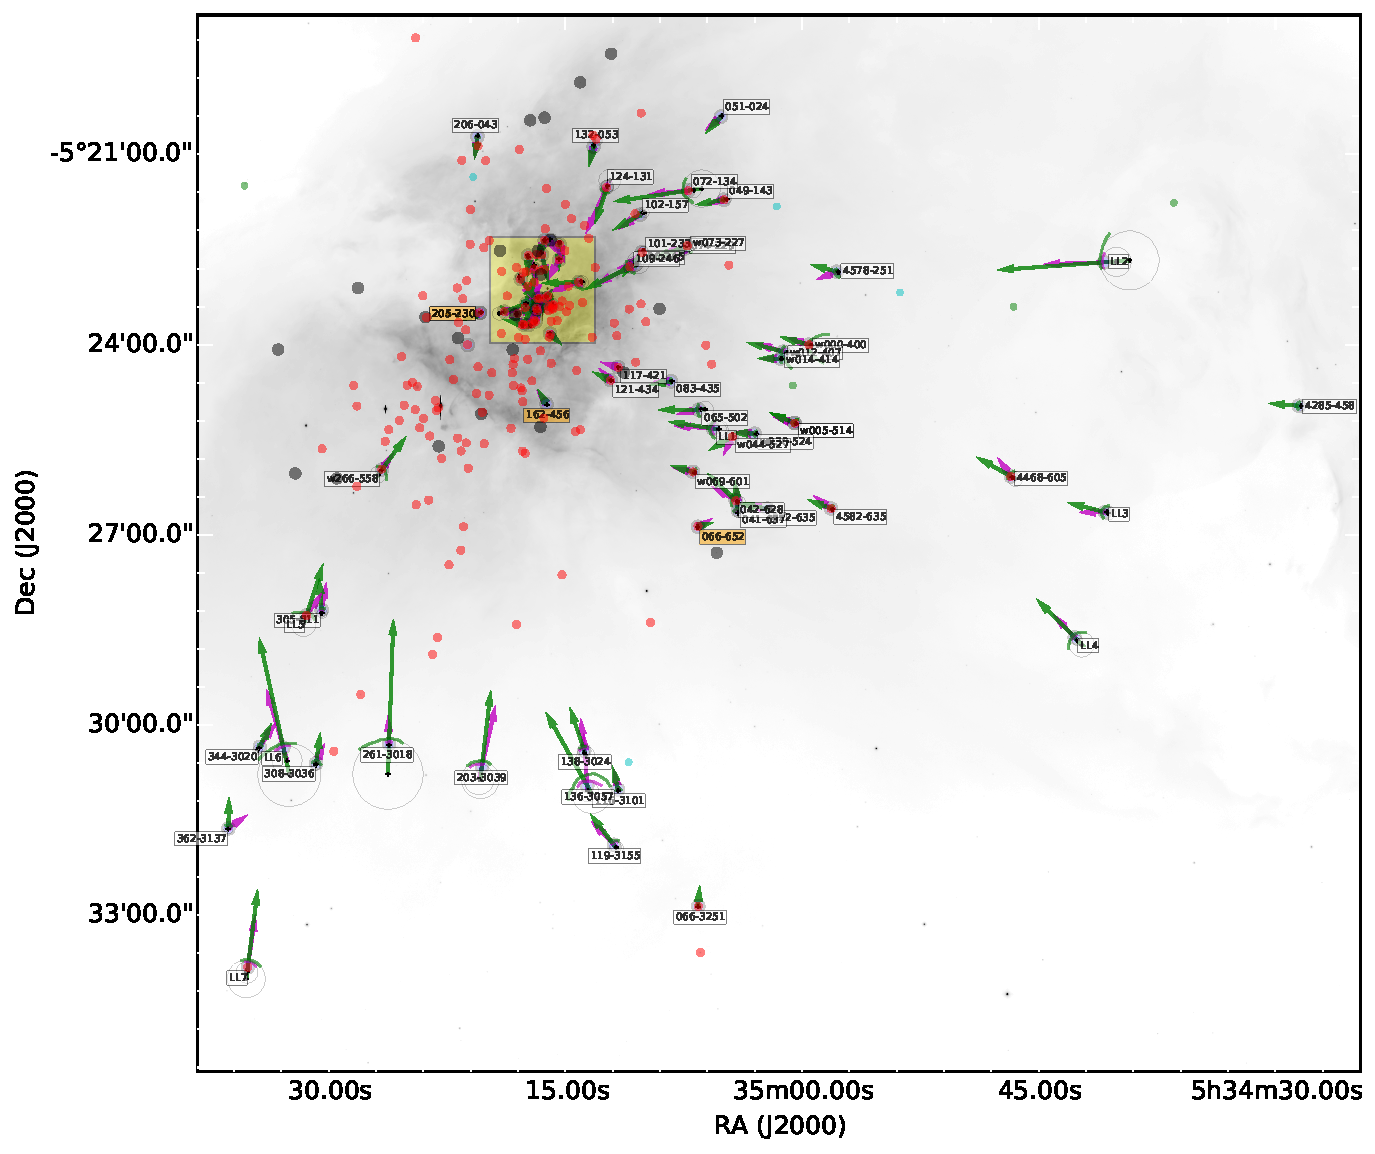
\includegraphics[width=\linewidth]{ll-pos-image}
  \caption{Position of bow shock arcs.}
  \label{fig:pos-image}
\end{figure*}

\begin{figure*}
  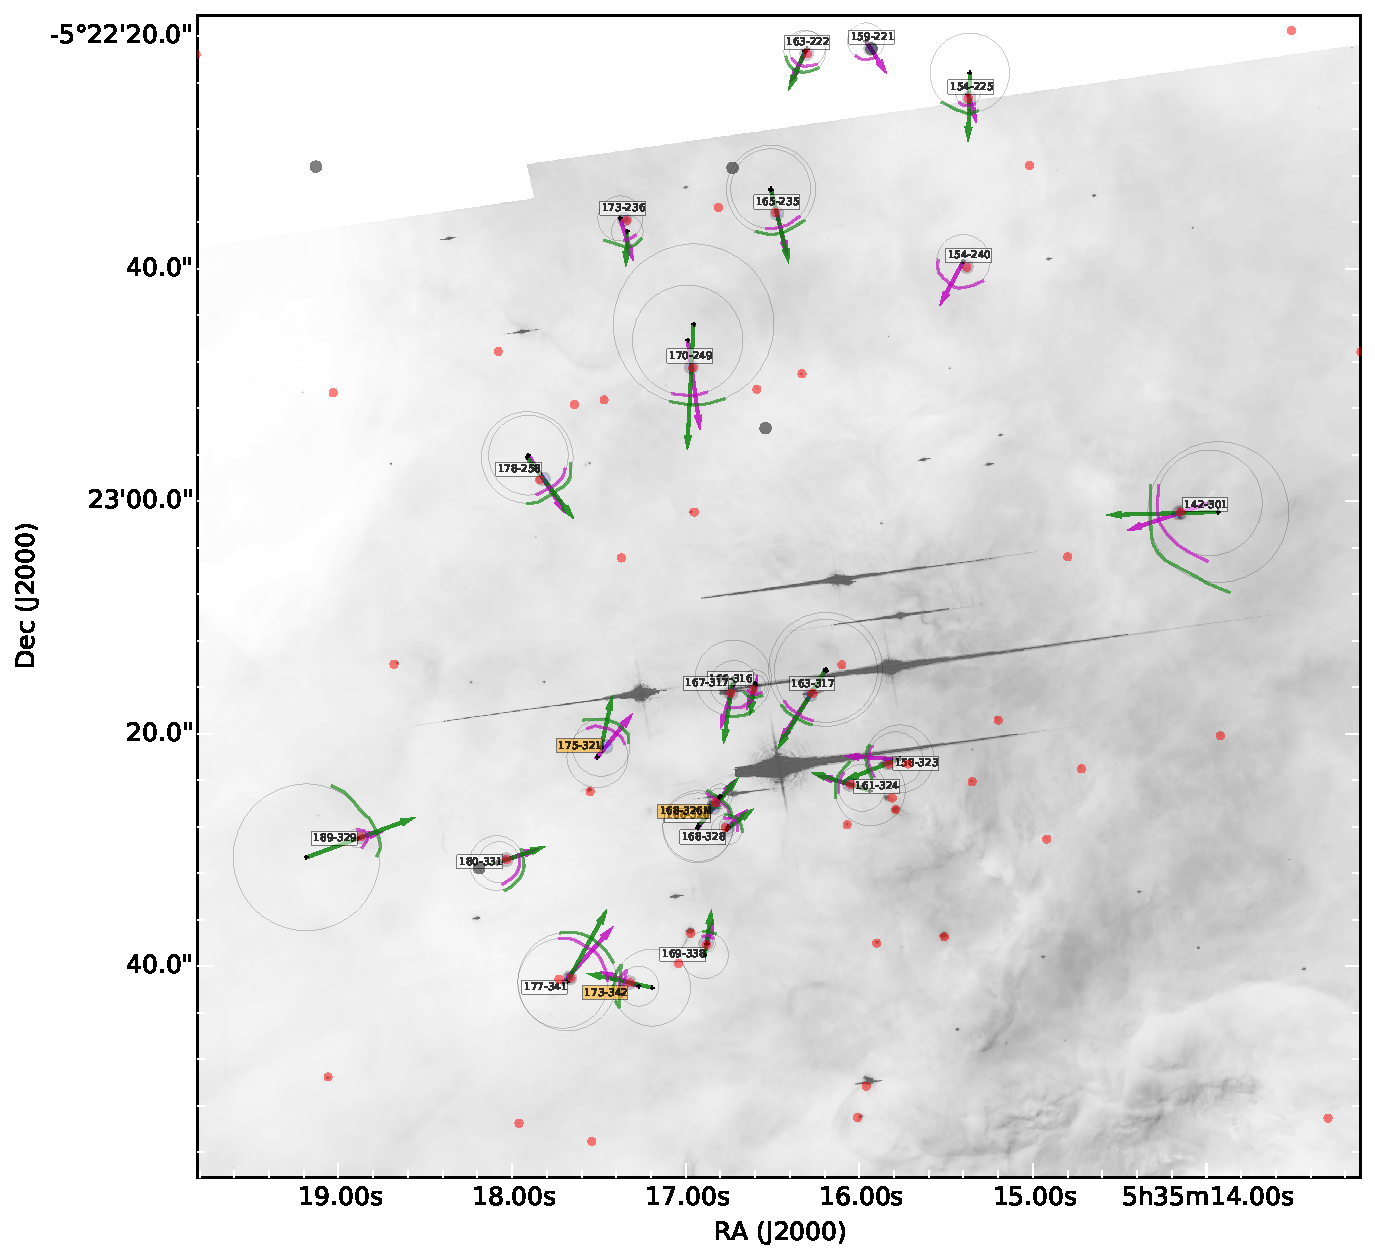
\includegraphics[width=\linewidth]{ll-pos-image-zoom}
  \caption{Position of bow shock arcs. Zoomed area.}
  \label{fig:pos-image}
\end{figure*}

\section{Catalog}
\label{sec:catalog}

\subsection{LV knot group}
\label{sec:lv-group}
\input{table-sort-01-LV.tex}
\input{fig-stamps-01-LV.tex}

\clearpage
\subsection{Southeast group}
\label{sec:se-group}
\input{table-sort-02-southeast.tex}
\input{fig-stamps-02-southeast.tex}

\clearpage
\subsection{North group}
\label{sec:n-group}
\input{table-sort-03-north.tex}
\input{fig-stamps-03-north.tex}

\clearpage
\subsection{Northwest group}
\label{sec:nw-group}
\input{table-sort-04-northwest.tex}
\input{fig-stamps-04-northwest.tex}

\clearpage
\subsection{Southwest group}
\label{sec:sw-group}
\input{table-sort-05-southwest.tex}
\input{fig-stamps-05-southwest.tex}

\clearpage
\subsection{West group}
\label{sec:w-group}
\input{table-sort-06-west.tex}
\input{fig-stamps-06-west.tex}

\clearpage
\subsection{South group}
\label{sec:s-group}
\input{table-sort-07-south.tex}
\input{fig-stamps-07-south.tex}

\clearpage
\subsection{Interproplyd shells}
\label{sec:interproplyd-group}
\input{table-sort-00-interproplyd.tex}
\input{fig-stamps-00-interproplyd.tex}

\clearpage
\section{Discussion}
\label{sec:discuss}
\begin{figure}
  (\textit{a})\\
  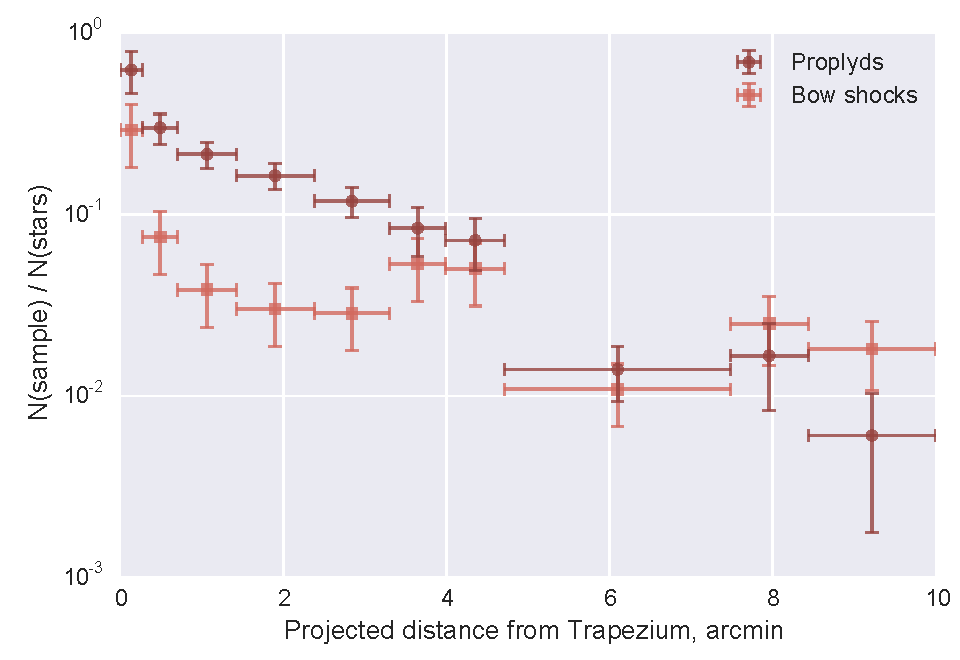
\includegraphics[width=\linewidth]{proplyd-star-ratio}\\
  (\textit{b})\\
  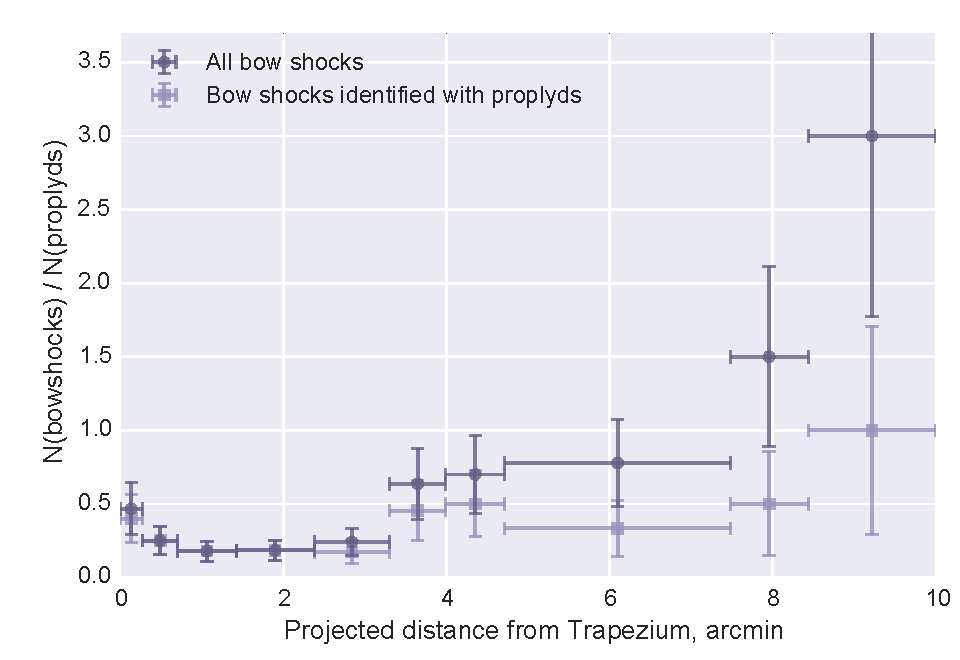
\includegraphics[width=\linewidth]{bowshock-proplyd-ratio}
  \caption{(\textit{a})~Fraction of all optically visible stars that
    are proplyds (dark circle symbols) or have bowshocks (light square
    symbols) as a function of projected separation from the Trapezium.
    (\textit{b})~Ratio between number of bowshocks and number of
    proplyds as a function of projected separation from the Trapezium.
    Dark circle symbols show all bowshocks in our catalog (with the
    exception of interproplyd shocks) while light square symbols show
    only those bowshocks associated with known or suspected proplyds.
  }
  \label{fig:bow-proplyd-star-ratios}
\end{figure}

Proplyd over star fraction falls off relatively smoothly with projected distance.  Albeit with a sudden drop after about 200 arcsec.


Bowshock over proplyd fraction seems to have three separate peaks.   Very small distances corresponding to the wind-wind interaction, then there is a dearth of bowshocks until a second peak around four arcmin.  Finally at very large radii there may be a third peak of objects that are not proplyds.

But an alternate explanation for the third peak could be that they are all proplyds but that the proplyd fraction is underestimated at large distances.

On the other hand there is also evidence for three distinct populations from the azimuthal distribution around the Trapezium.  The group at 4 arcmin separation are mainly to the west whereas the more distant objects are mainly to the south.


\end{document}
